\section{Metodologia}

O presente experimento foi desenvolvido com o objetivo de simular um sistema de modulação e demodulação em frequência (FM) utilizando o ambiente GNU Radio.

\subsection{Geração do Sinal FM}

A geração do sinal FM foi realizada a partir de um sinal senoidal com frequência de 1 kHz, representando o sinal de mensagem. Esse sinal foi conectado a um bloco \textbf{VCO (Voltage Controlled Oscillator)}, cuja frequência central foi configurada para 10 kHz.

O VCO gera um sinal cuja \textbf{frequência instantânea varia proporcionalmente à amplitude da senoide}, de acordo com a equação:

\begin{equation}
f_i(t) = f_c + k_f \cdot m(t)
\end{equation}

onde:
\begin{itemize}
    \item $f_i(t)$ = frequência instantânea;
    \item $f_c$ = frequência central da portadora (10 kHz);
    \item $k_f$ = sensibilidade de frequência do VCO, configurada como $2\pi \cdot f_c$;
    \item $m(t)$ = sinal de mensagem (senoide de 1 kHz).
\end{itemize}

Para permitir o ajuste dinâmico da amplitude do sinal de mensagem, foi utilizado um bloco \textbf{QT GUI Range}, com os seguintes parâmetros:
\begin{itemize}
    \item \textbf{Start}: 0
    \item \textbf{Stop}: 100 m
    \item \textbf{Step}: 2 m
    \item \textbf{Name}: amp
\end{itemize}

O controle da amplitude é fundamental, pois ela impacta diretamente no \textbf{desvio de frequência} ($\Delta f$) do sinal FM e, consequentemente, no \textbf{índice de modulação} ($\beta$), definido como:

\begin{equation}
\beta = \frac{\Delta f}{f_m}
\end{equation}

\noindent
sendo $f_m$ a frequência do sinal de mensagem (1 kHz).

Além disso, um bloco \textbf{Add Const} foi inserido com valor 1, garantindo que o sinal de entrada no VCO não assuma valores negativos, o que poderia causar deslocamentos indesejados na frequência portadora.

\begin{figure}[!h]
    \centering
    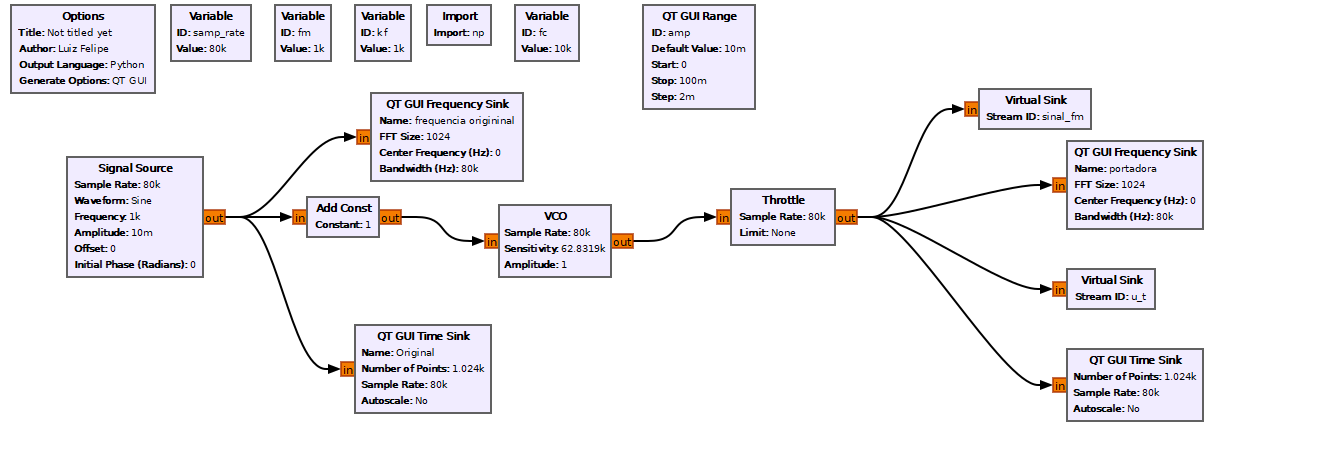
\includegraphics[width=0.5\textwidth]{images/FM_FLUXOGRAMA.png}
    \caption{Fluxograma do processo de modulação e demodulação FM.}
    \label{fig:fluxograma}
\end{figure}

\subsection{Demodulação do Sinal FM}

A recuperação do sinal de mensagem a partir do sinal FM foi realizada por meio da seguinte sequência de blocos:

\begin{enumerate}
    \item \textbf{Hilbert Transform}: o sinal real do VCO é convertido em um sinal complexo, gerando uma representação em banda unilateral. Este processo permite separar a informação de fase, necessária para demodulação baseada em frequência. O filtro de Hilbert foi configurado com \textbf{65 taps}, valor escolhido como compromisso entre resposta em frequência adequada e baixa distorção de fase, uma vez que um número maior de taps melhora a precisão, mas aumenta a latência.

    \item \textbf{Quadrature Demod}: esse bloco realiza a diferenciação da fase entre amostras consecutivas, estimando assim a \textbf{frequência instantânea}, proporcional ao sinal de mensagem. Sua operação é descrita matematicamente por:

    \begin{equation}
    y[n] = \frac{\mathrm{arg}\left( x[n] \cdot \overline{x[n-1]} \right)}{2\pi}
    \end{equation}

    O parâmetro de ganho foi configurado como:

    \begin{equation}
    \mathrm{Ganho} = \frac{\text{samp\_rate}}{2\pi \cdot f_c}
    \end{equation}

    Este fator de escala garante que o sinal demodulado corresponda numericamente à amplitude do sinal de mensagem, normalizando a saída de acordo com a frequência da portadora. Em termos práticos, esse ganho ajusta a sensibilidade do detector para converter variações de fase (em radianos) em variações proporcionais de frequência (em Hz) e, por consequência, em amplitude do sinal de mensagem.

    \item \textbf{Multiply Const}: etapa de ajuste fino na escala do sinal demodulado, permitindo calibrar a amplitude conforme desejado para comparação com o sinal original.

    \item \textbf{DC Block}: remove componentes de média (offset DC) que podem estar presentes após a demodulação. Esse offset geralmente é introduzido por imperfeições no processamento de fase e precisa ser removido para que o sinal tenha referência centrada em zero.

    \item \textbf{Filtro Passa-Baixa}: remove ruídos de alta frequência presentes na saída do quadrature demod, além de eliminar componentes residuais fora da banda do sinal de interesse. A configuração utilizada foi:
    \begin{itemize}
        \item \textbf{Frequência de corte}: 1.5 kHz, ligeiramente acima da frequência máxima do sinal de mensagem (1 kHz), garantindo a preservação total do conteúdo útil;
        \item \textbf{Largura de transição}: 500 Hz, proporcionando uma boa atenuação fora da banda sem exigir um filtro excessivamente complexo.
    \end{itemize}
\end{enumerate}

\begin{figure}[!h]
    \centering
    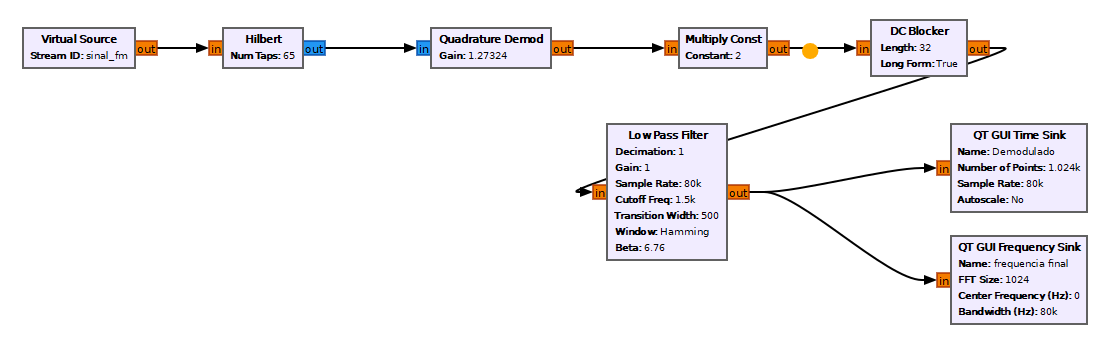
\includegraphics[width=0.5\textwidth]{images/DEM_FM.png}
    \caption{Diagrama de blocos da demodulação FM.}
    \label{fig:demodulacao}
\end{figure}


\subsection{Justificativa dos Parâmetros Escolhidos}

Os parâmetros foram definidos levando em consideração os seguintes critérios técnicos:

\begin{itemize}
    \item \textbf{Frequência de portadora (10 kHz)}: suficiente para separar a banda do sinal FM da baseband, permitindo uma representação clara da modulação.
    \item \textbf{Frequência de mensagem (1 kHz)}: escolhida para facilitar a visualização dos efeitos da modulação, estando confortavelmente abaixo da portadora.
    \item \textbf{Sensibilidade do VCO (2$\pi$ $\cdot$ 10k)}: essa escolha permite que a variação de fase no sinal FM corresponda diretamente à variação da amplitude do sinal de mensagem, alinhando os conceitos teóricos com a implementação prática.
    \item \textbf{Hilbert com 65 taps}: número suficiente para garantir boa precisão na conversão para sinal analítico sem exigir demasiada carga computacional.
    \item \textbf{Filtro passa-baixa com 1.5kHz}: protege contra aliasing e remove ruídos fora da banda, mantendo integralmente o conteúdo do sinal original.
\end{itemize}
